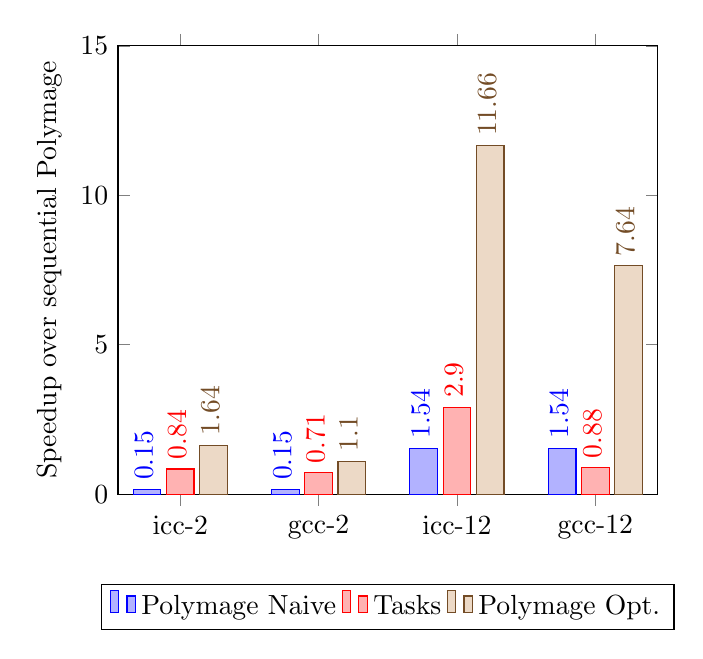
\begin{tikzpicture}
  \centering
  \begin{axis}[
    ybar,
    enlargelimits=0.15,
    enlarge y limits=false,
    ymin=0,
    ymax=15,
     legend style={at={(0.5,-0.2)},
        anchor=north,legend columns=-1},
        ylabel={Speedup over sequential Polymage},
        symbolic x coords={icc-2,gcc-2,icc-12,gcc-12},
      xtick=data,
        nodes near coords,
    every node near coord/.append style={
        anchor=mid west,
        rotate=90
    }
    ]
    \addplot coordinates {(icc-2,0.15)(gcc-2,0.15)(icc-12,1.54)(gcc-12,1.54)};
    \addplot coordinates {(icc-2,0.84)(gcc-2,0.71)(icc-12,2.9)(gcc-12,0.88)};
    \addplot coordinates {(icc-2,1.64)(gcc-2,1.1)(icc-12,11.66)(gcc-12,7.64)};
    \legend{Polymage Naive, Tasks, Polymage Opt.}
  \end{axis}
\end{tikzpicture}